\subsection*{Actividad 2}

Consumo de heladeras, según clase, por hora. 

\begin{center}
\begin{tabular}{ccccc}
Horas & A     & C   & D   & E   \\ \hline
0     & 0     & 0   & 0   & 0   \\
1     & 26.5  & 41  & 50  & 59  \\
2     & 53    & 82  & 100 & 118 \\
3     & 79.5  & 123 & 150 & 177 \\
4     & 106   & 164 & 200 & 236 \\
5     & 132.5 & 205 & 250 & 295 \\
6     & 159   & 246 & 300 & 354 \\ \hline
\end{tabular}
\end{center}

Esta tabla de datos se puede representar gráficamente:

\begin{align*}
	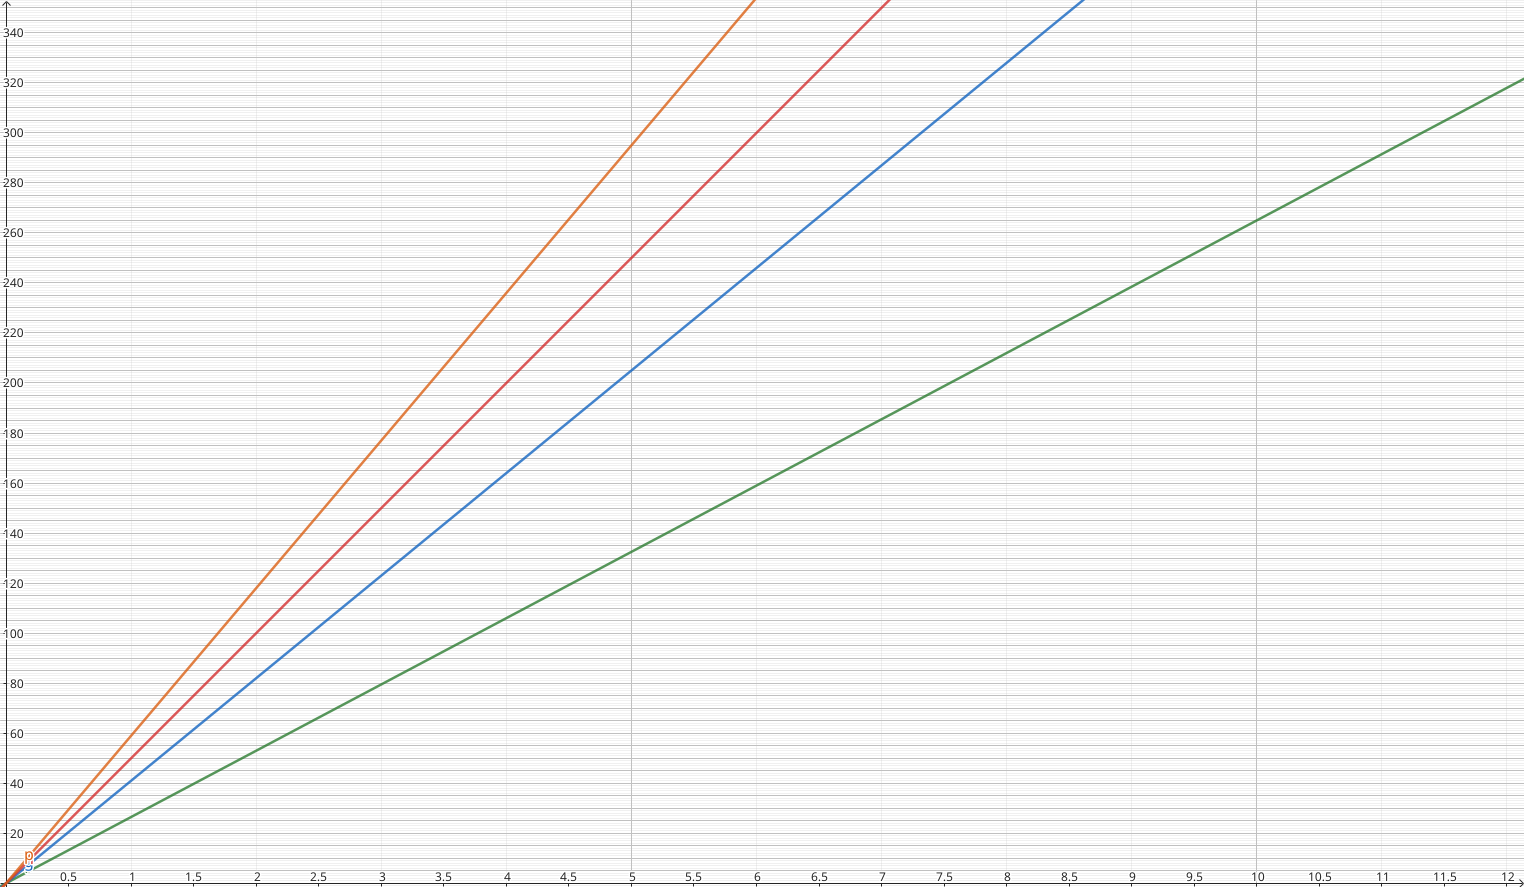
\includegraphics[scale=.4]{02/actividad2/img/heladeras2}
\end{align*}

Las función de consumo en vatios por hora de uso de cada clase de heladera es:

\begin{align*}
	A(x) &= 26.5x\\ 
	C(x) &= 41x\\ 
	D(x) &= 50x\\ 
	E(x) &= 59x
\end{align*}

La pendiente de cada función indica el consumo por hora de cada clase de heladera.

Una heladera de clase A consume 636 vatios por día, mientras una heladera clase E consume 1416 vatios por día. Usar una heladera clase A permite ahorrar hasta un 55%.

